Figure~\ref{fig:goal_scenariotype} compared goal completion scores under different scenario types across different models.
In general, models are more likely to achieve social goals in smaller environments, yet the difference is relatively small, especially for larger models.
Qwen2.5-14b, compared with other models, has shown the most balanced performance, especially superseding GPT-4o in large society scenarios.

\begin{figure*}
    \centering
    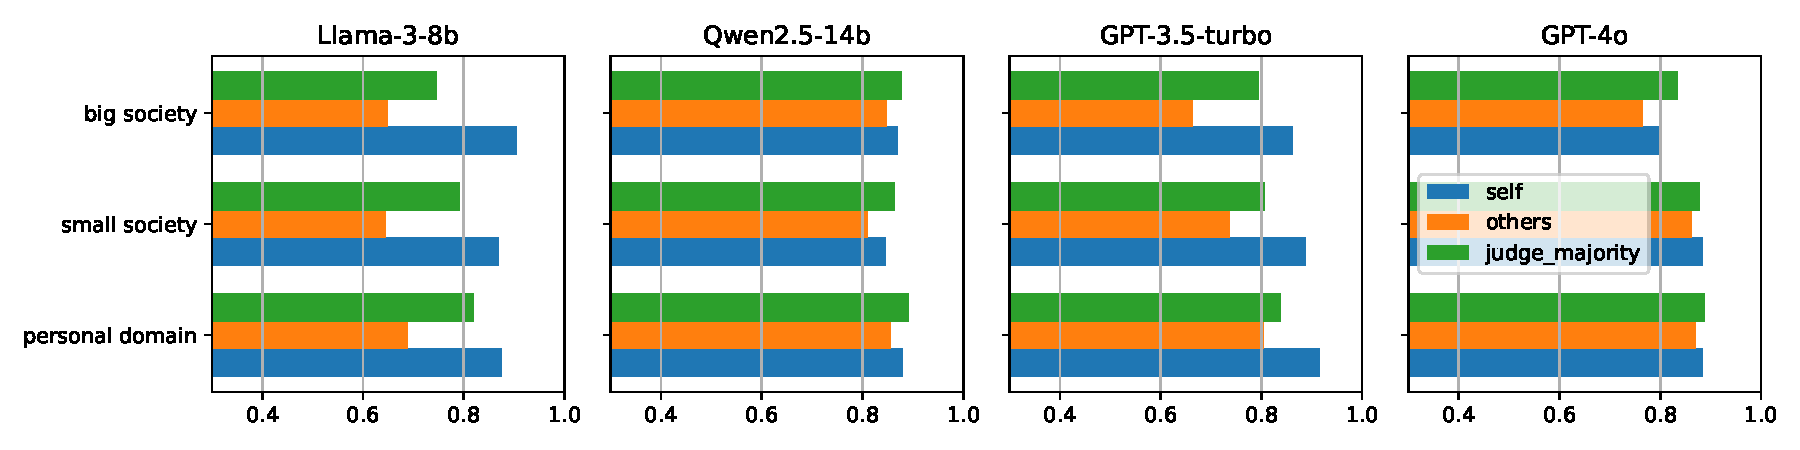
\includegraphics[width=\textwidth]{latex/figs/goal_scenetype.pdf}
    \caption{Goal completion scores under different scenario types across models.}
    \label{fig:goal_scenariotype}
\end{figure*}

Figure~\ref{fig:goal_nrounds} demonstrates how goal completion scores change as we increase the number of interacting rounds.
It appears that there is no best number of rounds regarding all three evaluation aspects (self, other and external), while the trends also vary between models.
Again, larger models are more robust to this factor, indicating that they can complete their demands in a few number of interactions while keep concentrated during the whole dialog.

\begin{figure*}
    \centering
    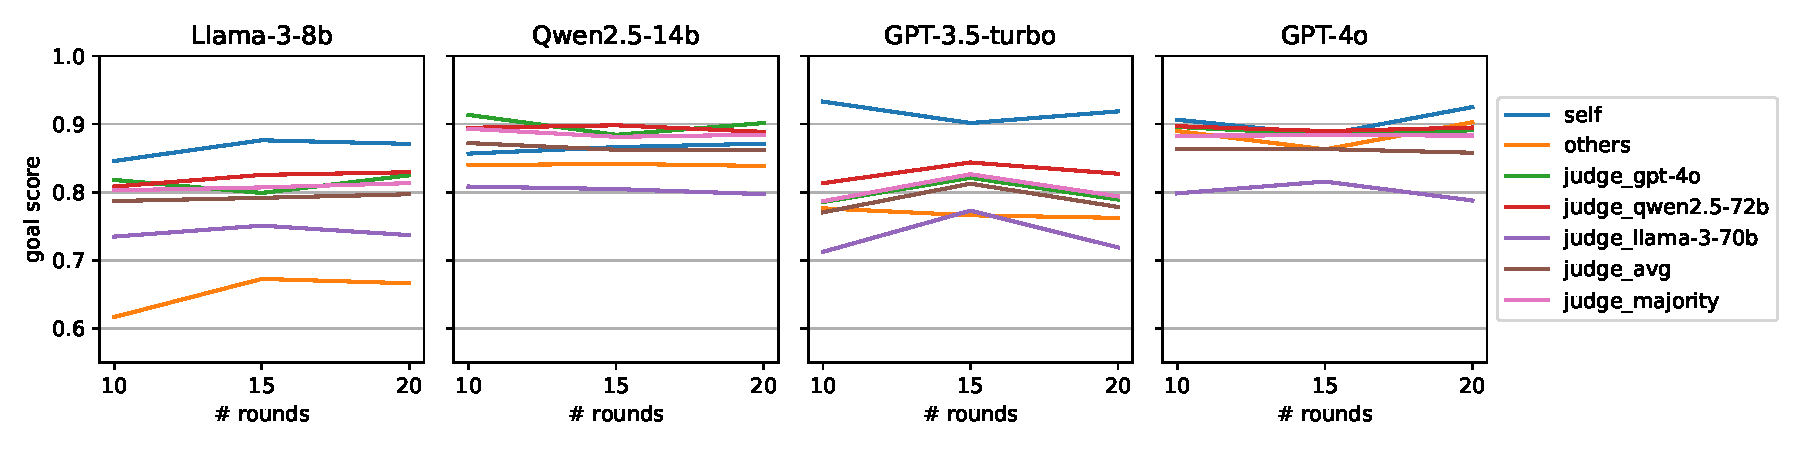
\includegraphics[width=\textwidth]{latex/figs/goal_nrounds.pdf}
    \caption{Goal completion scores under different number of rounds across models.}
    \label{fig:goal_nrounds}
\end{figure*}

Figure~\ref{fig:goal_nagents} illustrates the relation between goal completion scores and the number of participants in the scenario.
As expected, social goals become harder to achieve when more agents are involved.
Note that in our benchmark, most 5-agent scenarios have relatively easy goals (e.g. a group of friends having a casual chat about a subject), leading to a higher average score than 4-agent scenarios.
Therefore, we claim that the type of the goals are more important than the number of agent when measuring the difficulty of a social scenario.

\begin{figure*}
    \centering
    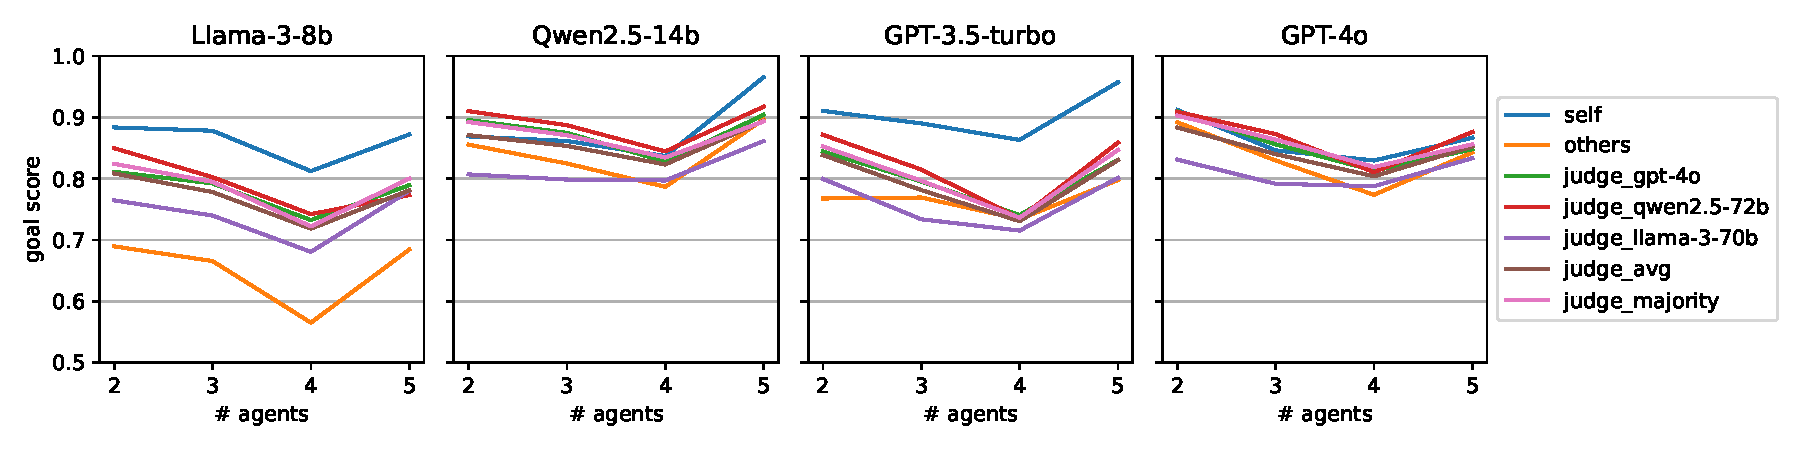
\includegraphics[width=\textwidth]{latex/figs/goal_nagents.pdf}
    \caption{Goal completion scores under different number of participants across models.}
    \label{fig:goal_nagents}
\end{figure*}